In some cases, the goal of a simulation is reproducing the macroscopic spiking activity
of a big network of neurons, diregarding the exact shape of a single action potential.
Therefore, sometimes it might be wise to simplify the model of a single neuron, such that
the overall computational cost becomes lighter and more feasible. In general, it can be
stated that the biological reliability - i.e., the shape of the action potential - is
inversely related to the computational efficiency, as shown in this scheme.
\begin{figure}[H]
    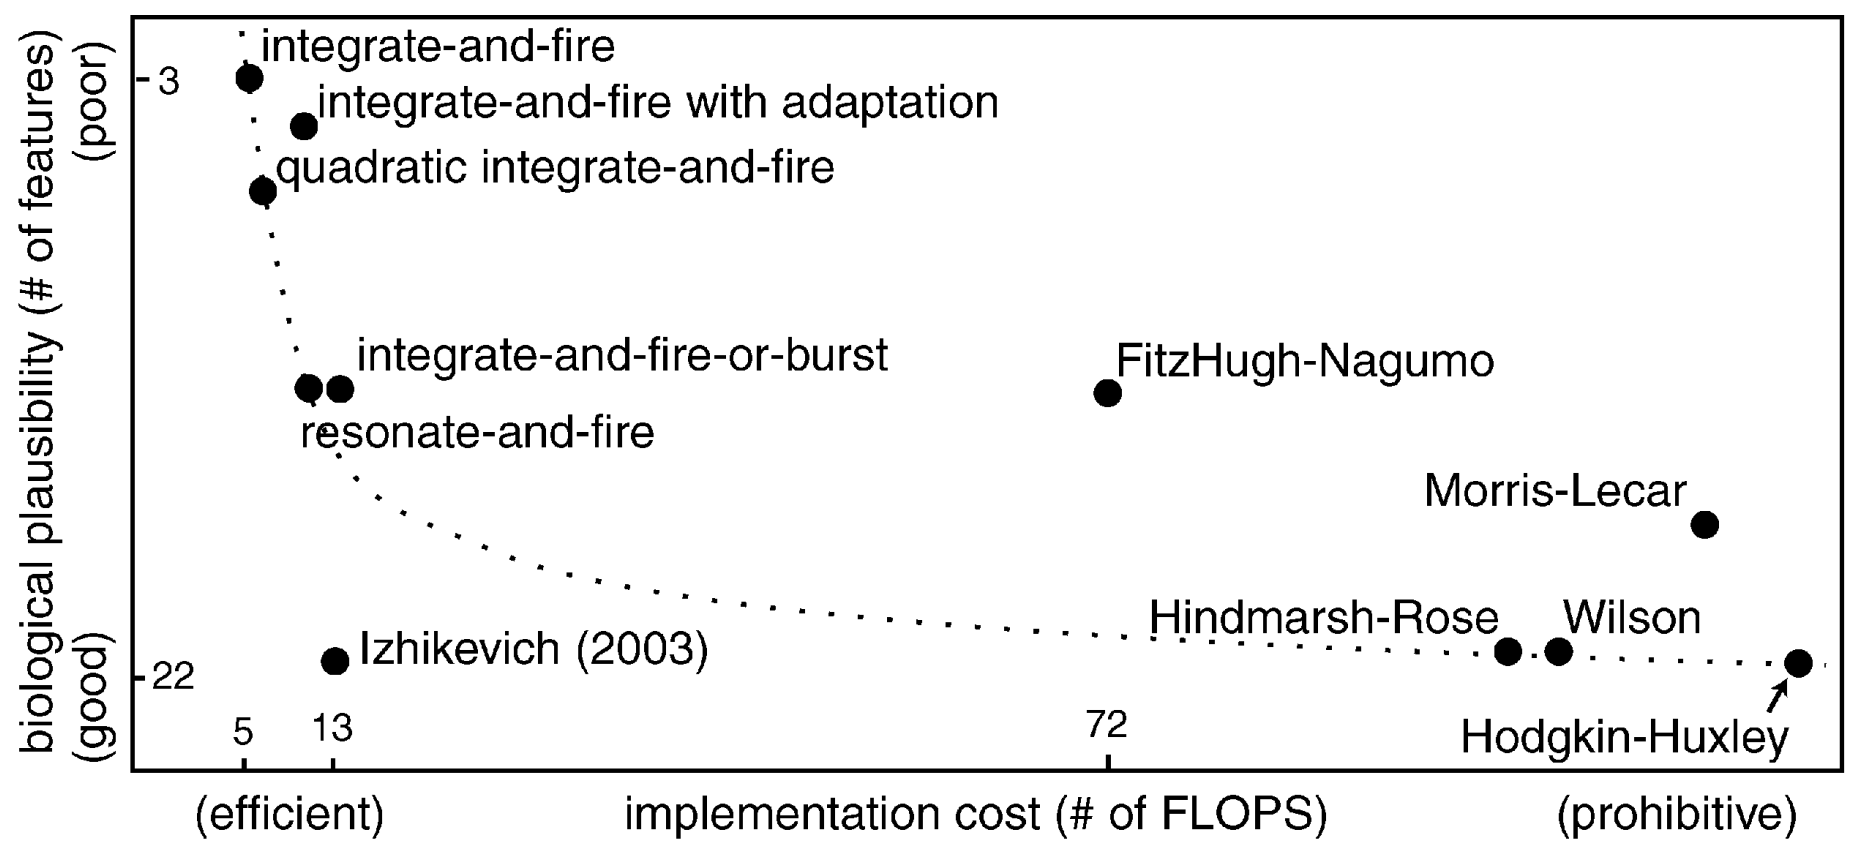
\includegraphics[scale=0.3]{10_1}
    \centering
\end{figure}

\subsection{Integrate-and-Fire Models}
The Integrate-and-Fire (IF) models are a class of abstract neuronal models extremely performant
from a computational point of view. The trade-off here is losing detail in the shape of the
action potential. These models are based on two steps: integration - i.e., the summation of the
input stimuli - and firing - i.e., the emission of a spike.\\
A bioinspired model behaves as shown below, all the input stimuli are integrated together,
both spatially and temporally, a depolarization occurs and whenever the excitability threshold
\(\theta\) is overcome, then an action potential is elicited.
\begin{figure}[H]
    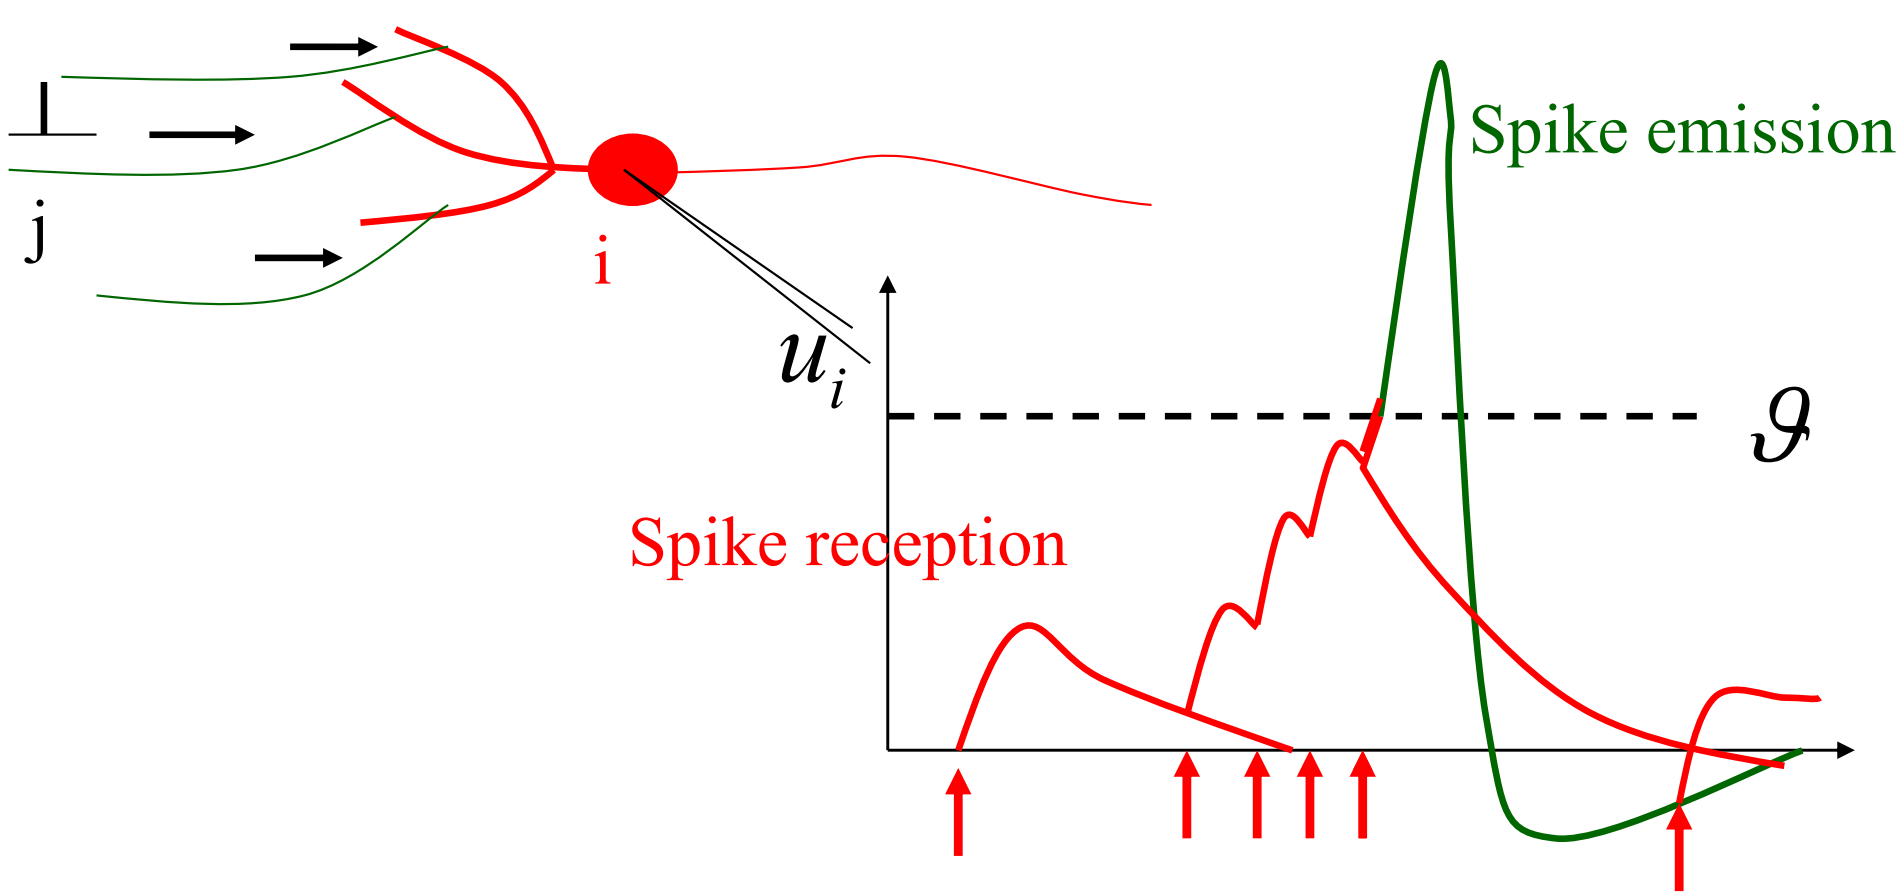
\includegraphics[scale=0.3]{10_2}
    \centering
\end{figure}
The IF models instead provides a temporal integration and aim at modelling what happens below the
excitability threshold, thus the inputs summation process. If the threshold is overcome, then
a spike is emitted and it is considered to be an instantaneous point process, thus a Dirac's delta.
After that, a reset time models the refractory period of the neuron, but the repolarization of the
membrane is not taken into account at all.
\begin{figure}[H]
    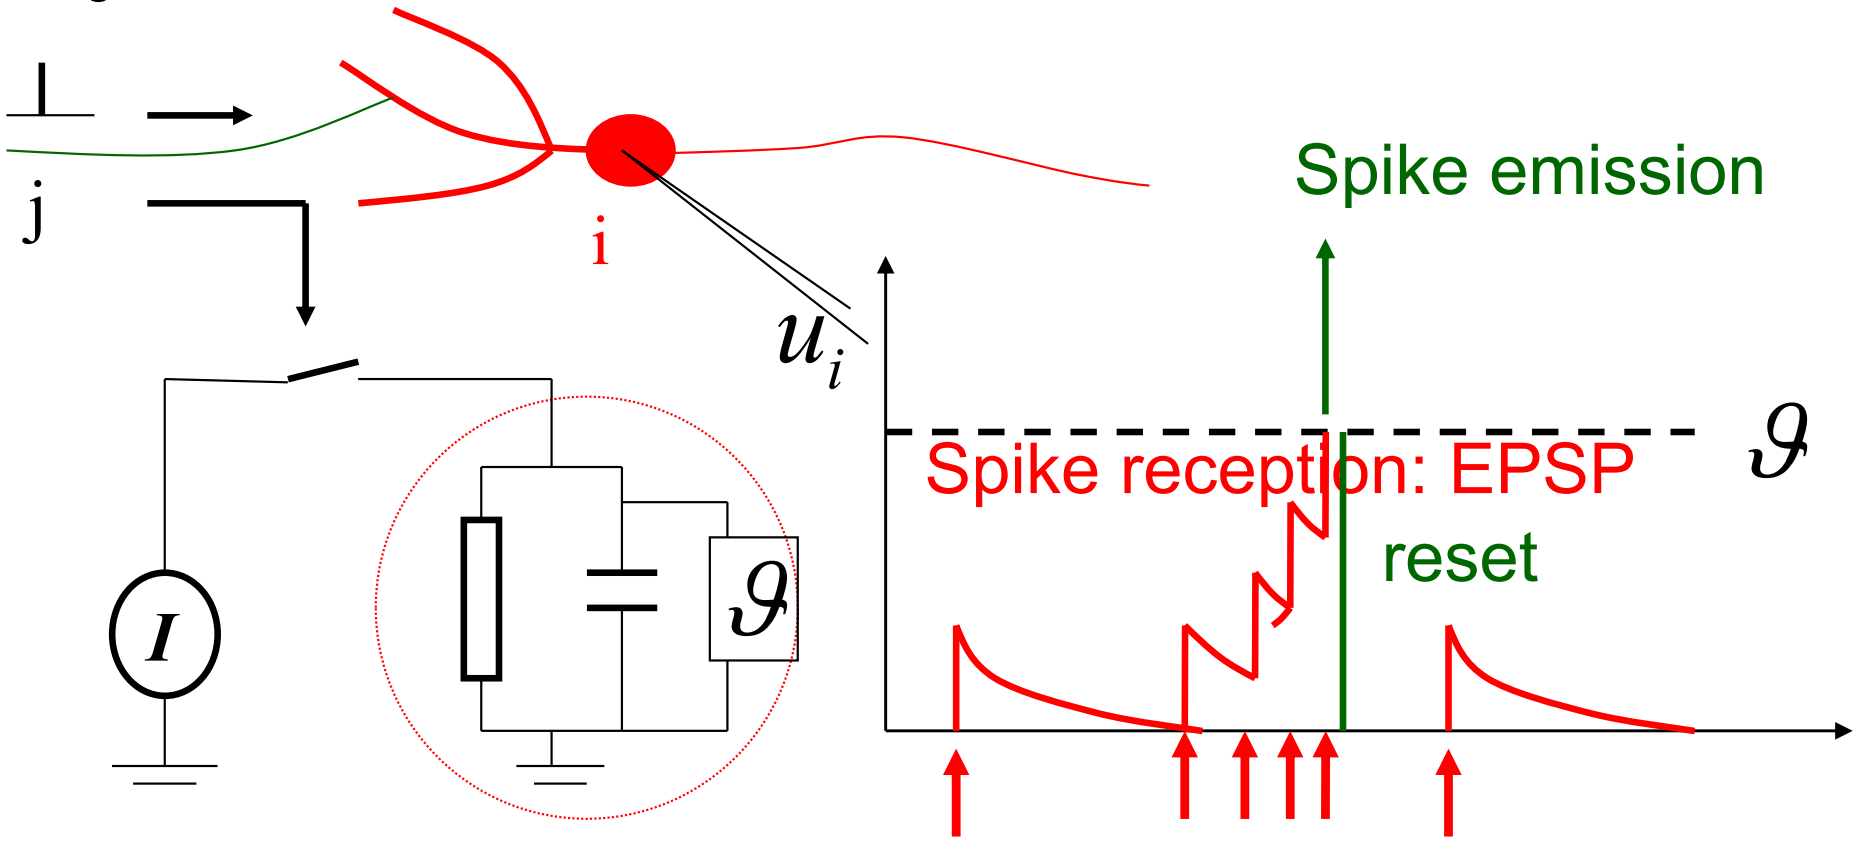
\includegraphics[scale=0.3]{10_3}
    \centering
\end{figure}
The state equation of the IF model is extremely simple:
\begin{equation*}
    C_{m}\frac{dV_{m}}{dt}=I_{app}(t)
\end{equation*}
When an input current is applied, the membrane potential increases until the excitability threhsold
\(V_{th}=\theta\) is reached, at that point a Dirac's delta spike is emitted and the voltage
immediately goes back to its resting value. Note that the firing frqeuency of the model increases
linearly without limits following the \(I_{app}\) increase. Often, a refractory period \(T_{ref}\)
is added, preventing the neuron to fire during that period. Thus, the firing frequency \(f(I_{app})\) is
a function of the input current \(I_{app}\) and can be computed as shown below.
\begin{equation*}
    C_{m}\frac{dV_{m}}{dt}=I_{app}(t)
    \Rightarrow
    C_{m}\int_{E_{rest}}^{V_{m}(t)}d\hat{V}=I_{app}(t)\int_{t_{0}}^{t}d\hat{t}
\end{equation*}
Let's assume \(E_{rest}=0\), \(t_{0}=0\) and a constant DC current pulse:
\begin{equation*}
    \Rightarrow
    V_{m}(t)=\frac{I_{app}}{C_{m}}t
    \Rightarrow
    T_{spike}=\frac{C_{m}V_{th}}{I_{app}}+T_{ref}=\frac{C_{m}V_{th}+T_{ref}I_{app}}{I_{app}}
\end{equation*}
Therefore, the spiking frequency is:
\begin{equation*}
    \Rightarrow
    f(I_{app})=\frac{1}{T_{spike}}=\frac{I_{app}}{C_{m}V_{th}+T_{ref}I_{app}}
\end{equation*}
\par
This model has a huge issue, as a matter of fact the capacitor \(C_{m}\) has no way to discharge but spiking,
therefore if the model receives a below-threshold signal at some time, it will retain that voltage boost forever
until it fires again. Thus, the model implement no time-dependent memory.
\subsubsection{Leaky-Integrate-and-Fire Neuron Model}
The absence of a discharging component affecting the standard IF model is hereby solved by by adding a leak term
to the membrane potential, reflecting the diffusion of ions through the membrane. Therefore, the state equation
is modified as:
\begin{itemize}
    \item \textbf{Sub-threshold behaviour} (\(V_{m}(t)<V_{th}\)):
          \begin{equation*}
              C_{m}\frac{dV_{m}}{dt}=-g_{leak}(V_{m}-E_{leak})+I_{app}
          \end{equation*}
    \item \textbf{Supra-threshold behaviour} (\(V_{m}(t^{*})\ge{V_{th}}\)):
          \begin{equation*}
              \begin{cases}
                  t^{*}\rightarrow{\text{a spike is registered}}=\sum_{k}\delta{(t-t_{k})} \\
                  V_{m}([t^{*};t^{*}+T_{ref}])=E_{rest}
              \end{cases}
          \end{equation*}
\end{itemize}
The equivalent circuit is modified as follow, by just adding a leakage resistor.
\begin{figure}[H]
    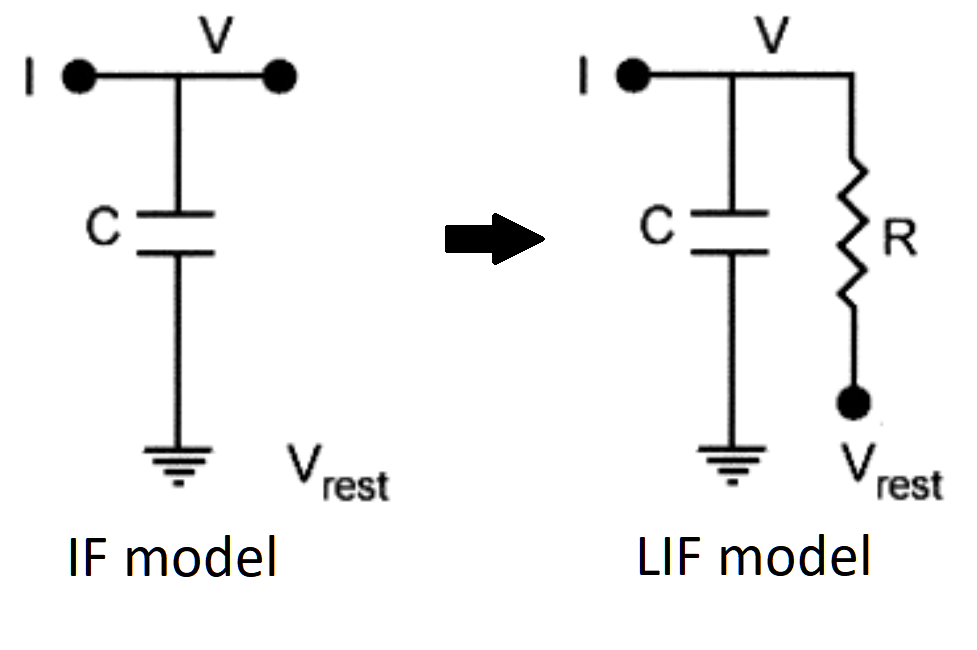
\includegraphics[scale=0.4]{10_4}
    \centering
\end{figure}
Without any applied input (\(I_{app}=0\)), the membrane potential is equal to the resting potential \(E_{rest}\).
On the contrary, if the integrated inputs leads to a membrane potential \(V_{m}\ge{V_{th}}\), then a spike is emitted.
After that, the voltage immediately goes to \(E_{rest}\) and remains at that value for a refractory period \(T_{ref}\).\\
Note that also in this case the shape of an action potential is diregarded and only its occurence in time is of interest,
as a matter of fact neural communication is based on the occurente time of spikes and not on their shape.\\
The firing frequency \(f(I_{app})\) of a LIF neuron can be found by solving the state equation:
\begin{equation*}
    C_{m}\frac{dV_{m}}{dt}=-g_{leak}(V_{m}-E_{leak})+I_{app}
    \Rightarrow
    V_{m}(t)=E_{rest}+R_{m}I_{app}(1-e^{-t/\tau_{m}})
\end{equation*}
By assuming \(E_{rest}=0\), let's set \(V_{m}(t)=V_{th}\):
\begin{equation*}
    V_{th}=R_{m}I_{app}(1-e^{-T_{spike}/\tau_{m}})
    \Rightarrow
    \frac{R_{m}I_{app}-V_{th}}{R_{m}I_{app}}=e^{-\frac{T_{spike}}{\tau_{m}}}
    \Rightarrow
    T_{spike}=\tau_{m}\ln{\Biggl(\frac{R_{m}I_{app}}{R_{m}I_{app}-V_{th}}\Biggr)}
\end{equation*}
Therefore, the firing frequency \(f(I_{app})\) is computed as:
\begin{equation*}
    f(I_{app})=\frac{1}{T_{spike}+T_{ref}}=\frac{1}{\tau_{m}\ln{\Biggl(\frac{R_{m}I_{app}}{R_{m}I_{app}-V_{th}}\Biggr)}+T_{ref}}
\end{equation*}
Note that the refractory period \(T_{ref}\) plays a critical role in limitating the maximum firing frequency of the model,
as depicted in the image below.
\begin{figure}[H]
    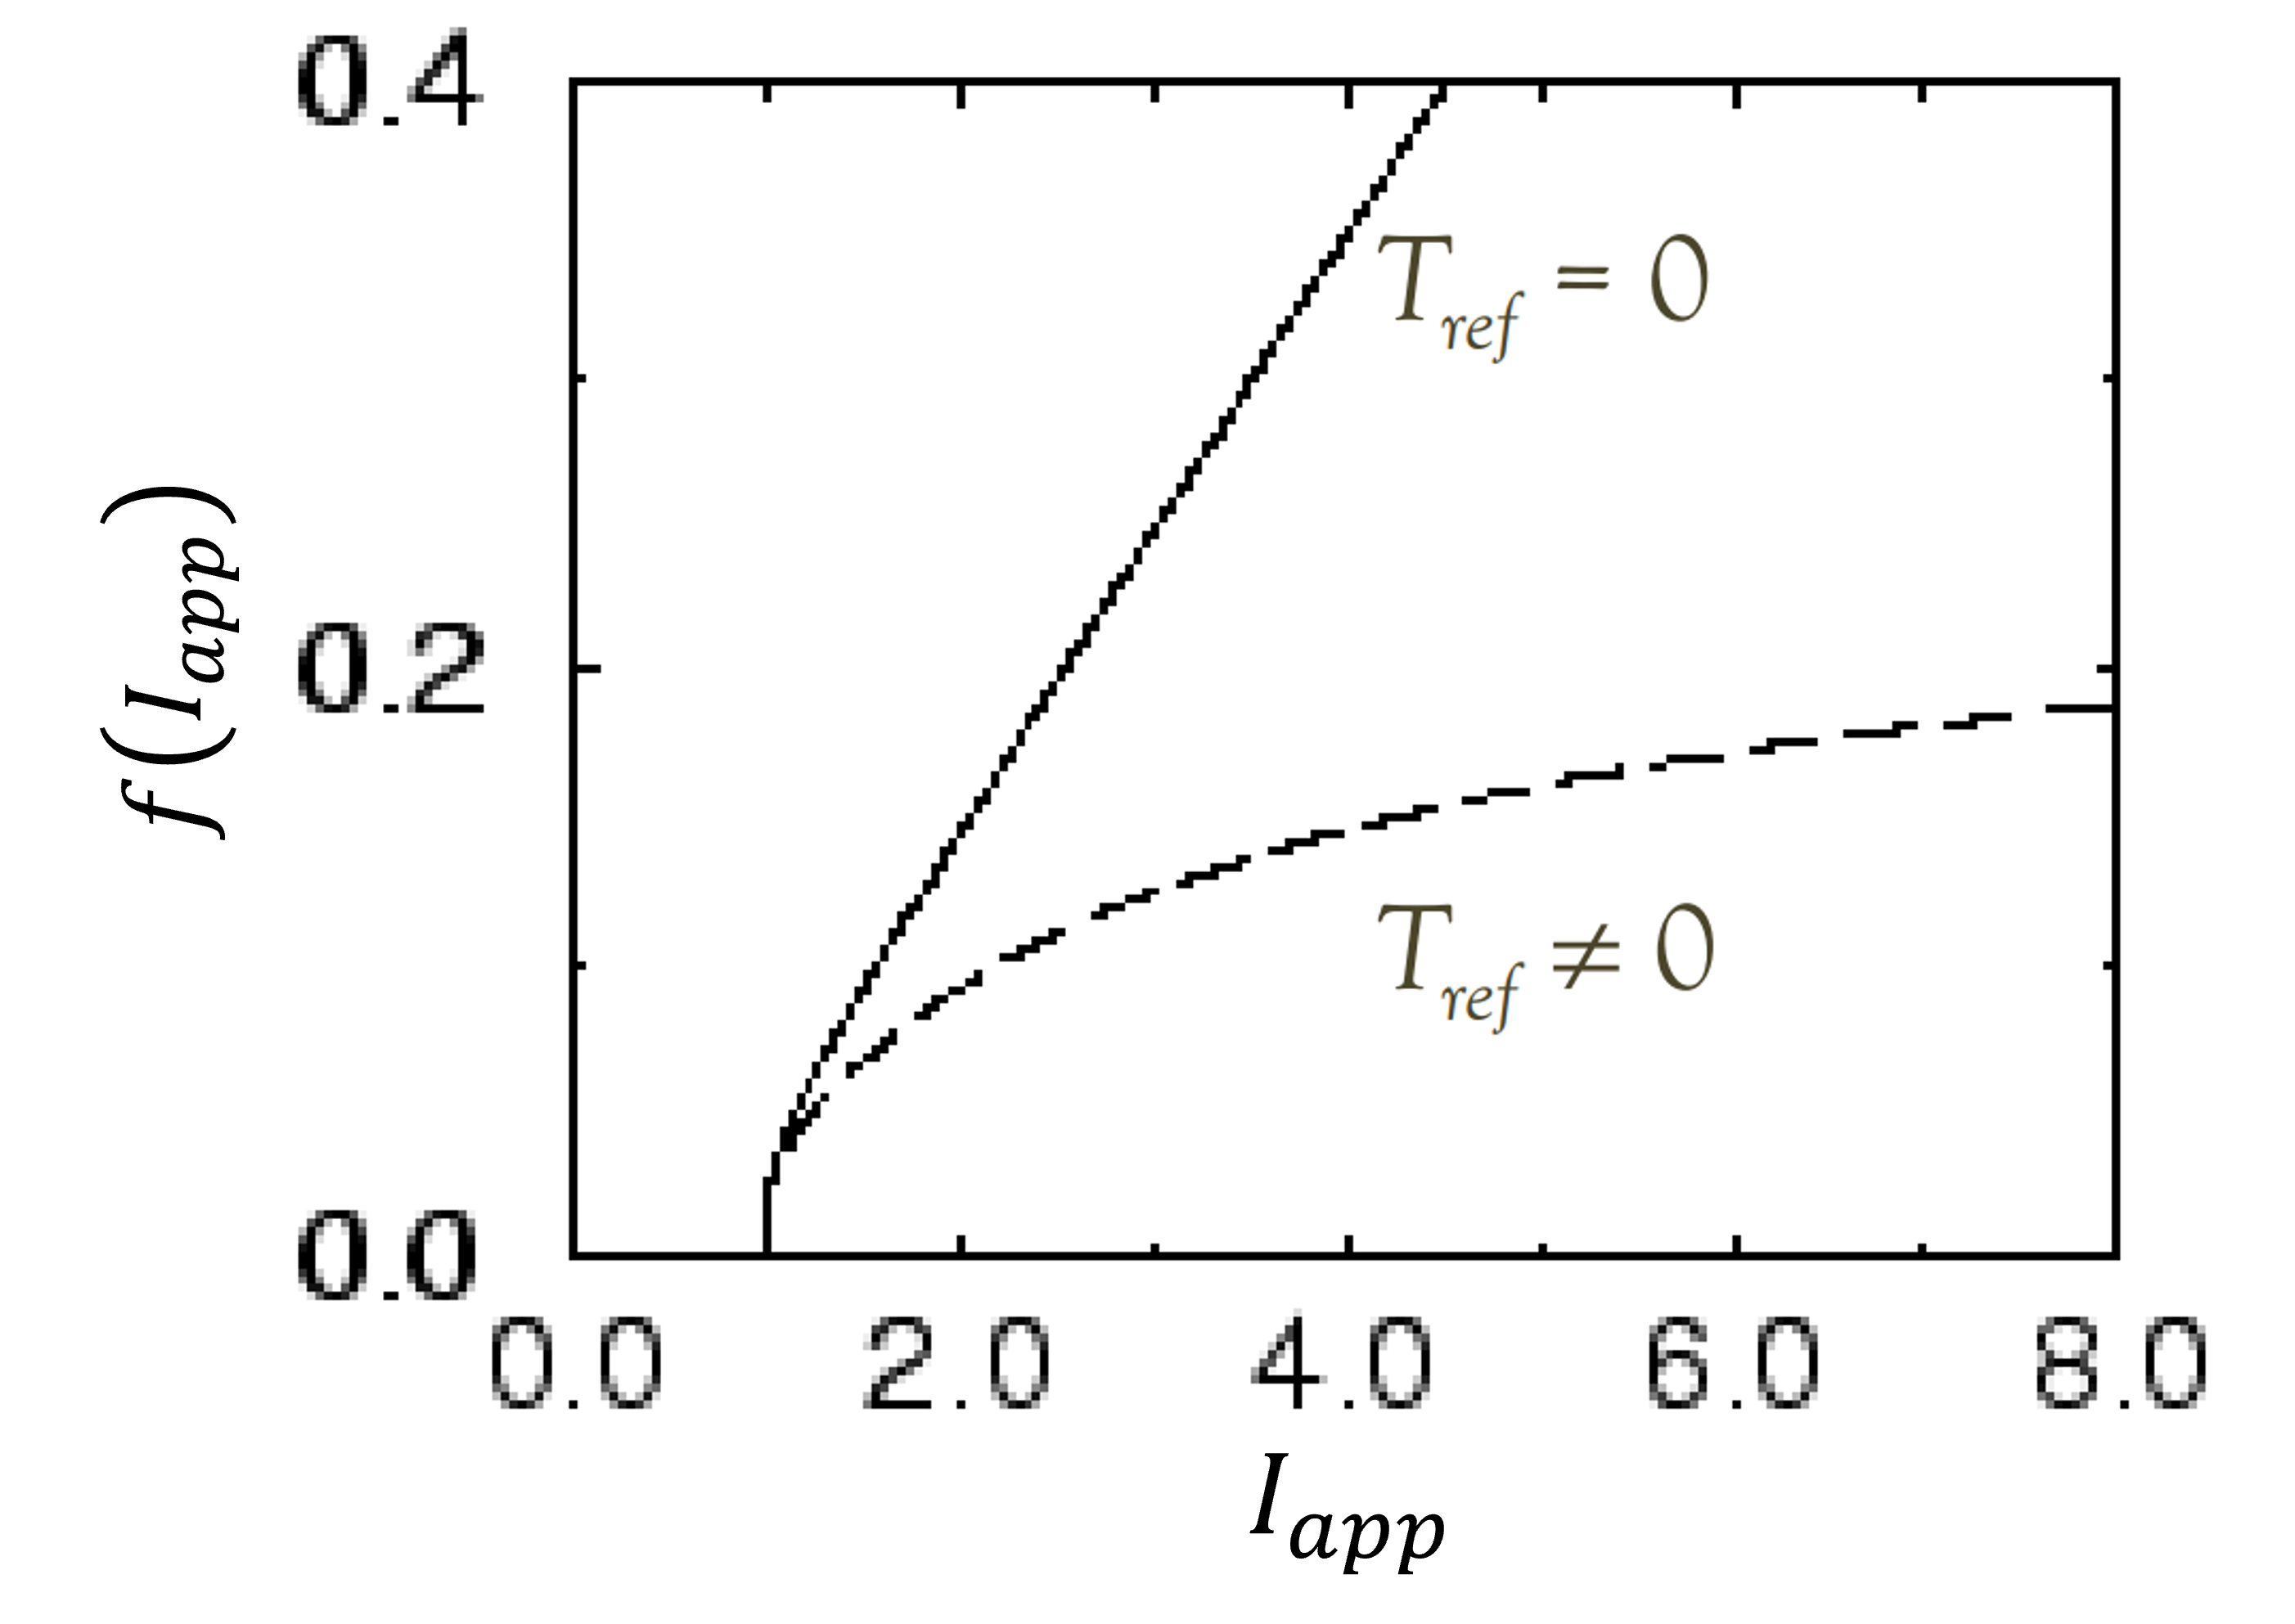
\includegraphics[scale=0.4]{10_5}
    \centering
\end{figure}
However, there are several types of dynamics not captured by the LIF model, in particular they are some kinds of
sub-threshold behaviours, the spike generation, the adaptation phenomenon, and the generation of bursts.
\subsubsection{Quadratic-Integrate-and-Fire Neuron Model}
In order to model certain patterns of activity, only two differential equations might not be sufficient,
however increasing their number might not be a proper solution, as a major requirement is to keep
low the computational cost. Henceforth, in some cases non-linearities are added to the state
equation such that more complex patterns are made available.\\
For instance the Quadratic-Integrate-and-Fire (QIF) model exploits a quadratic non-linearity to roughly model
the shape of an action potential, in particular its depolarization. Therefore, the model state equation is:
\begin{equation*}
    C_{m}\frac{dV_{m}}{dt}=-g_{leak}(V_{m}-E_{leak})+\psi(V_{m})+I_{app}
\end{equation*}
with the non-linearity being
\begin{equation*}
    \psi(V_{m})=\frac{g_{leak}}{2\Delta_{t}}(V_{m}-E_{T})^{2}+g_{leak}(V_{m}-E_{leak})-I_{T}
\end{equation*}
where \(\Delta_{T}\) is inversely related to the strength of the non-linearity and \(I_{T}\) is the
current threshold.
\begin{figure}[H]
    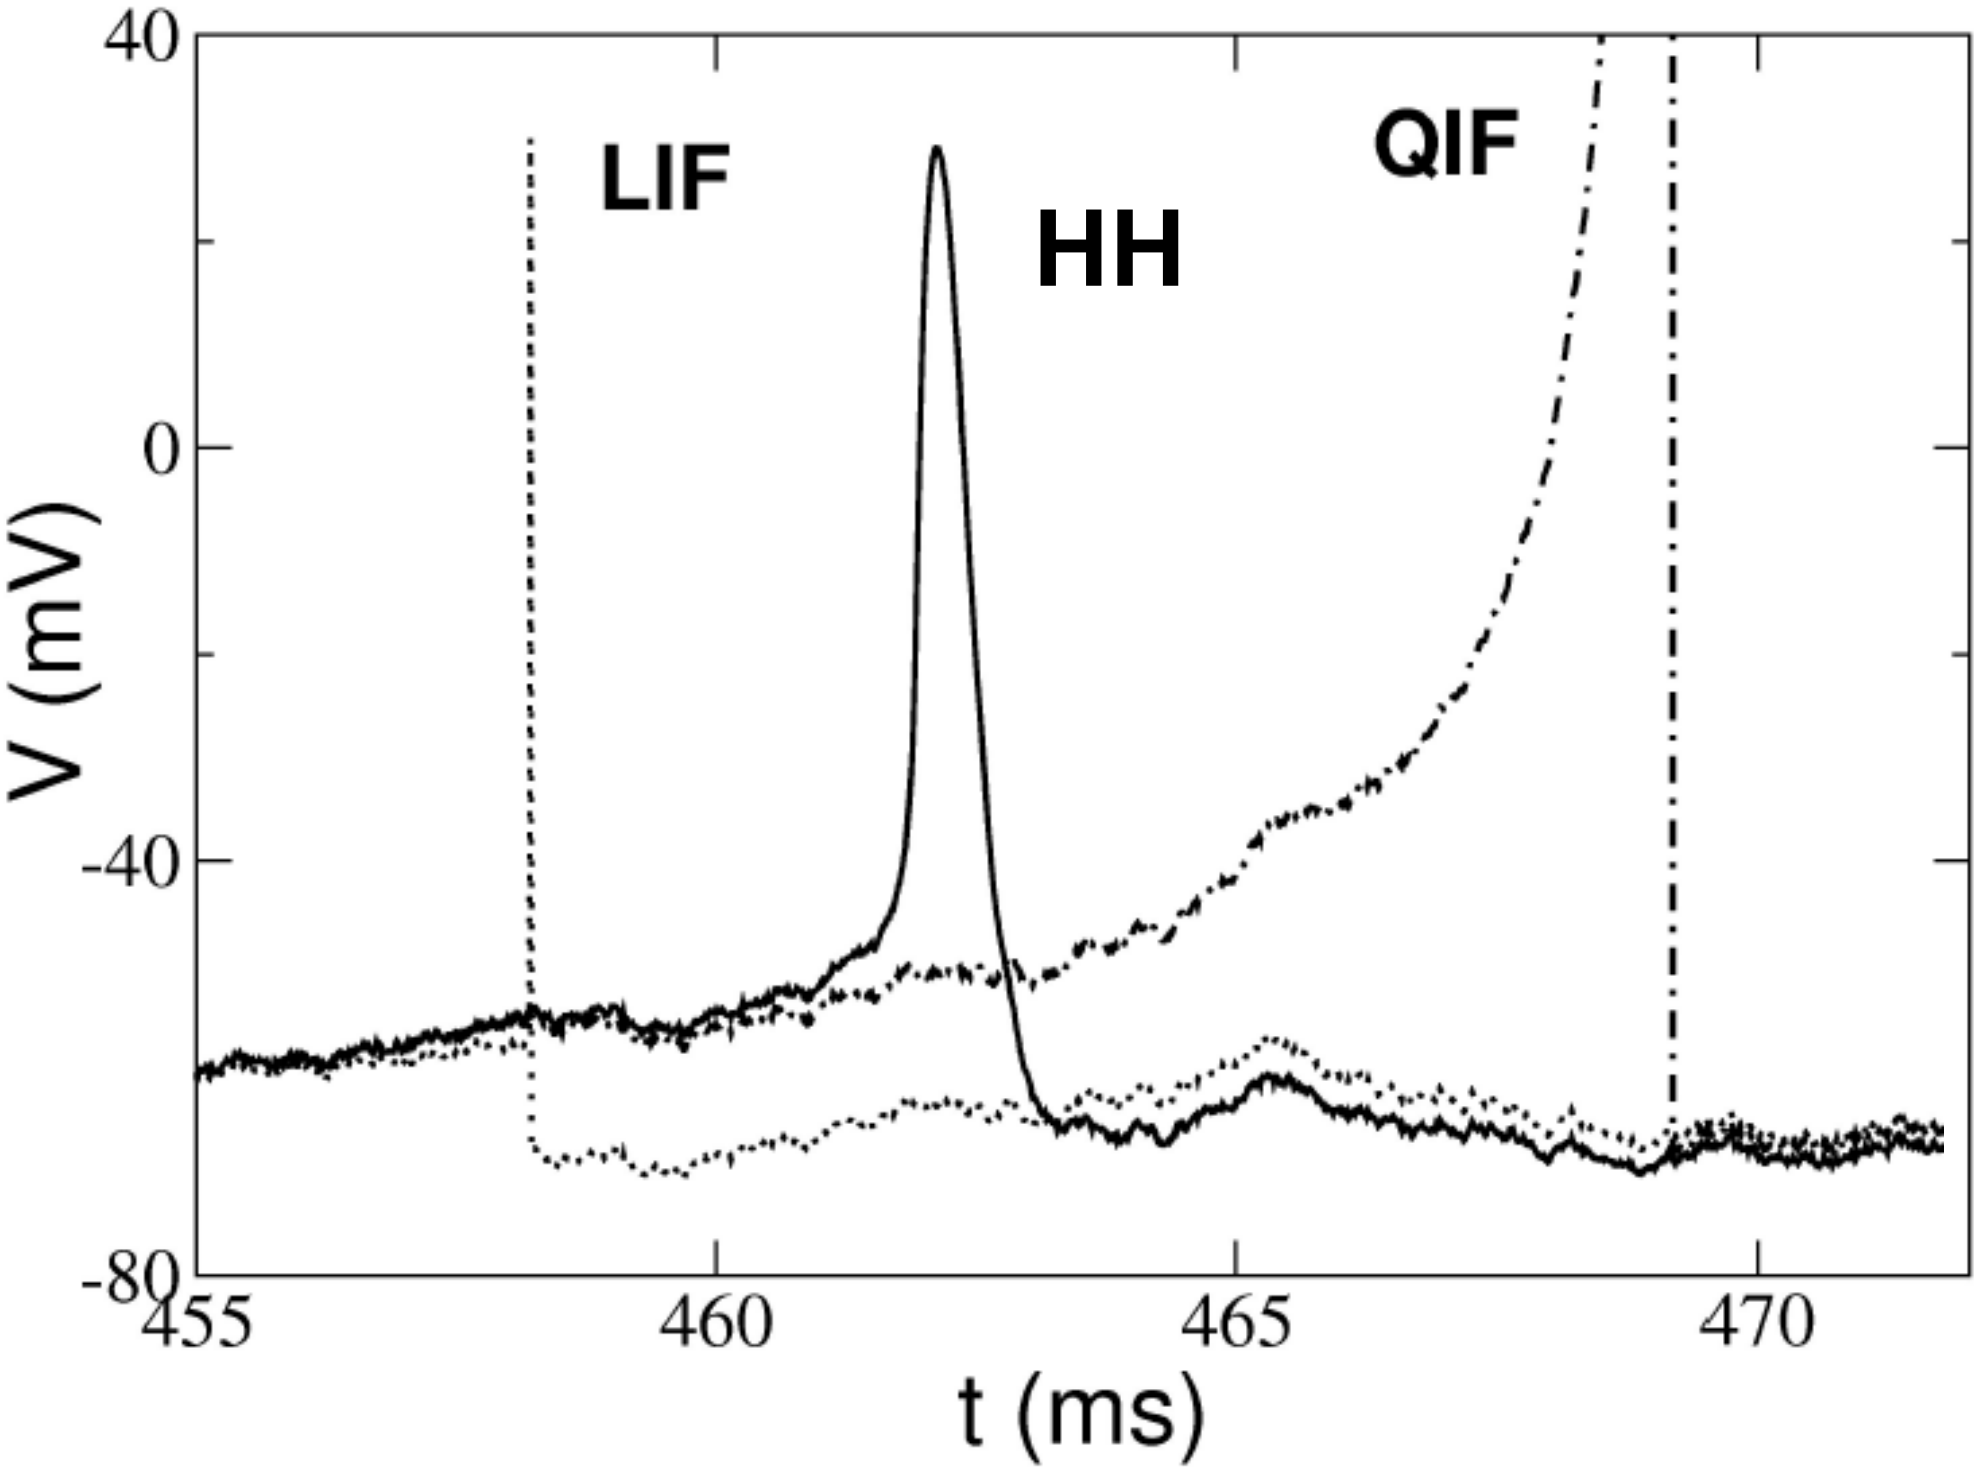
\includegraphics[scale=0.12]{10_6}
    \centering
\end{figure}
Unluckily, this solution introduces a delay in the generation of the spike with respect to the Hodgkin-Huxley model,
which is employed as a benchmark. Note that this delay may lose some spikes whenever they are tightly packed.
\subsubsection{Exponential-Integrate-and-Fire Neuron Model}
To mitigate the delay observed in the QIF model, a very similar model called Exponential-Integrate-and-Fire (EIF)
has been introduced. It has basically the same state equation, but it changes the non-linearity \(\psi(V_{m})\),
which is no longer quadratic, but an exponential-like term:
\begin{equation*}
    \psi(V_{m})=g_{leak}\Delta_{T}e^{\frac{V_{m}-E_{T}}{\Delta_{T}}}
\end{equation*}
\begin{figure}[H]
    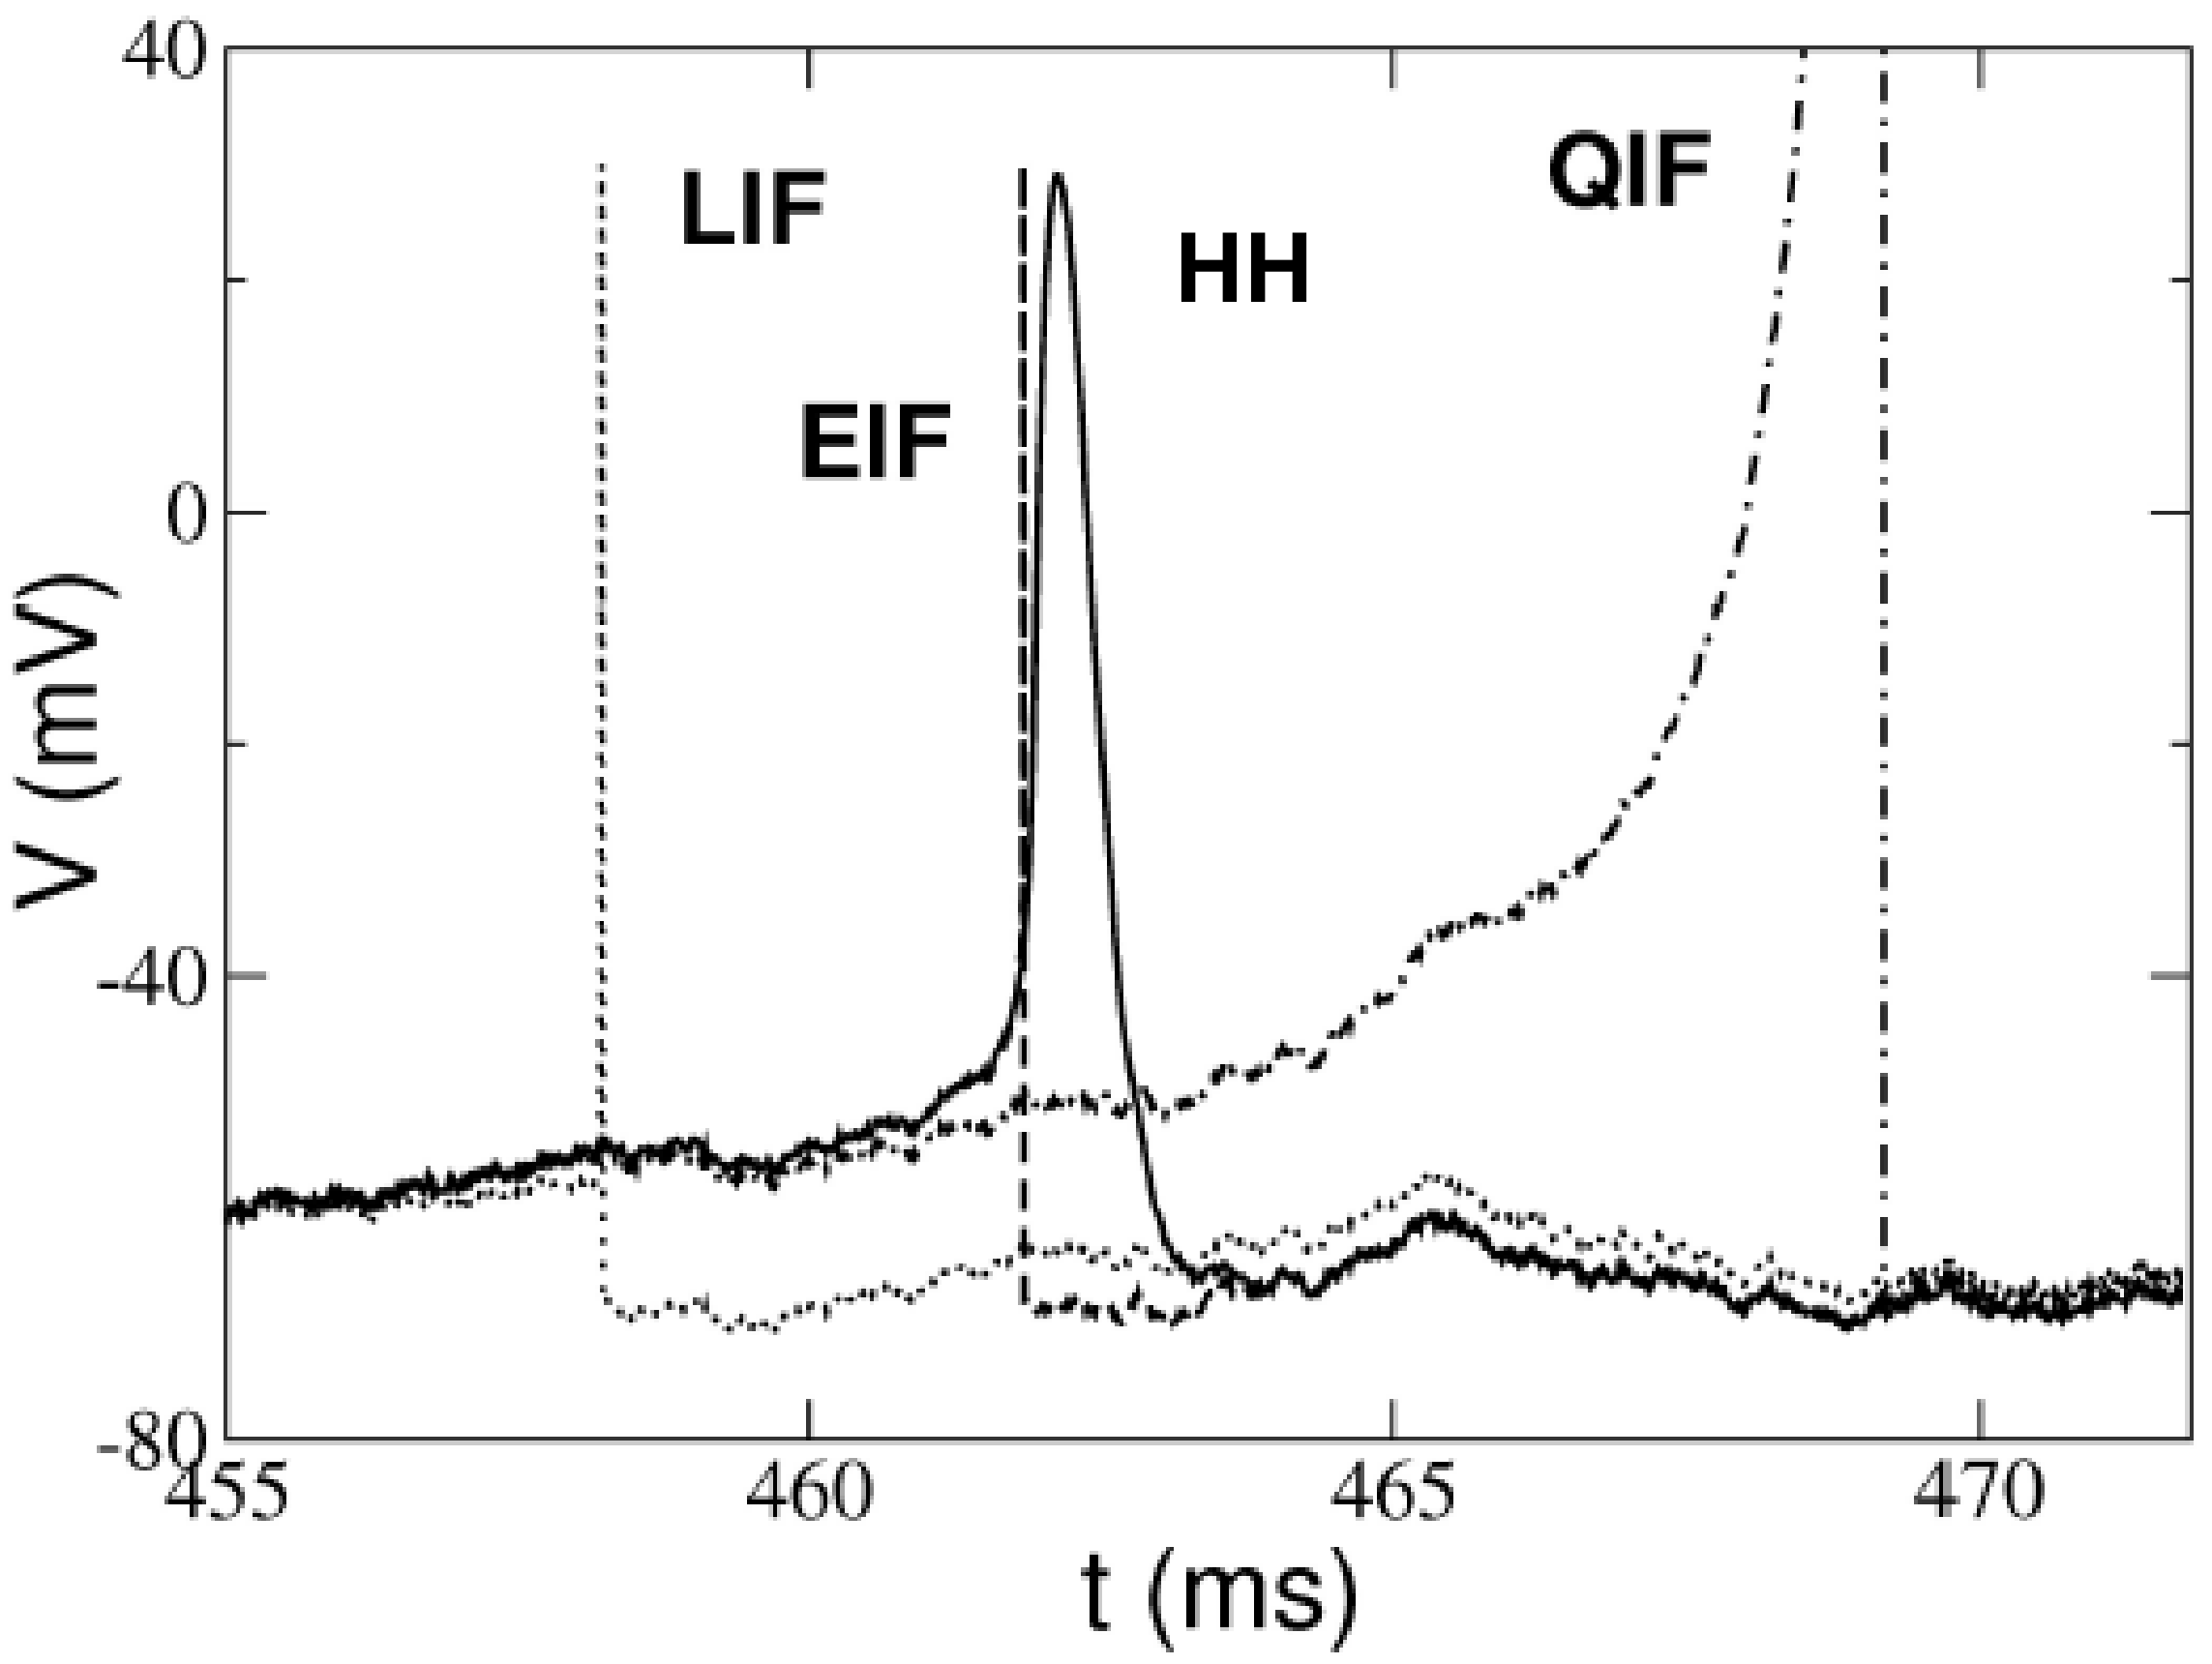
\includegraphics[scale=0.10]{10_7}
    \centering
\end{figure}
\par
Finally, all the models presented in the previous pages can be compared by looking at how they respond
to the same stimulus:
\begin{figure}[H]
    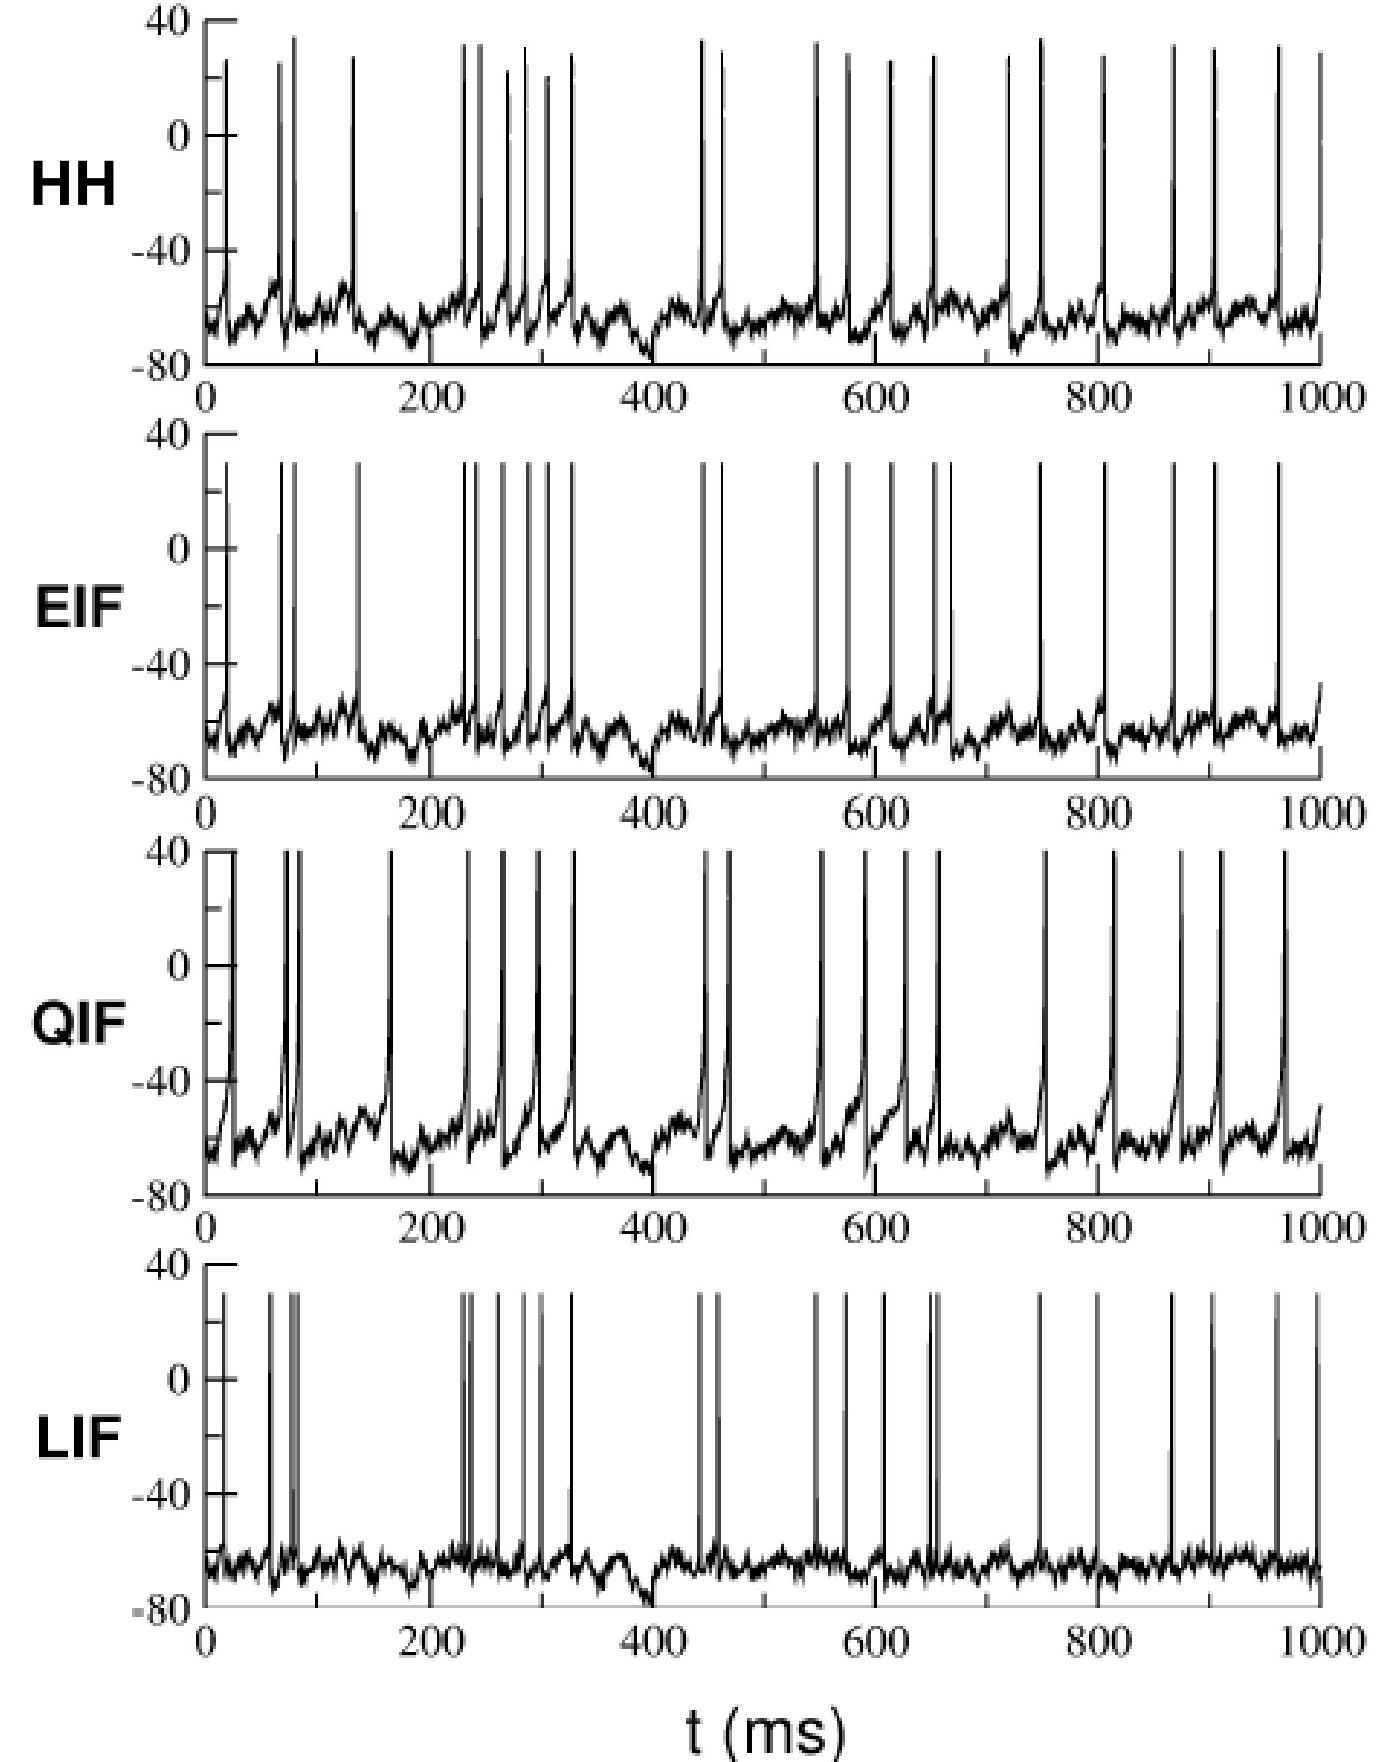
\includegraphics[scale=0.19]{10_8}
    \centering
\end{figure}
All the models seem to work in a similar way from a macroscopic point of view. Note that, as already said,
the QIF model tends to exhibit a slight delay and, because of being slower, it may lose some spikes
when they are packed together. As a consequence, all the models are characterized by a similar
firing rate \(f(I_{app})\) being a function of the applied current, but the QIF neuron's one will
be slightly lower, due to the missed spikes, especially when \(I_{app}\) and \(f(I_{app})\) increase.
\subsubsection{Integrate-and-Fire-or-Burst Neuron Model}
The Integrate-and-Fire-or-Burst (IFB) model is characterized by a double behaviour: it can both
elicit spikes and display bursting activity. To switch from one mode to the other, a biologically
meaningless function \(h\) is introduced in the state equation:
\begin{equation*}
    C_{m}\frac{dV_{m}}{dt}=-g_{leak}(V_{m}-E_{leak})-g_{T}\Theta(V_{m}-E_{h})h(V-E_{T})+I_{app}
\end{equation*}
The dynamics of the \(h\) function is:
\begin{equation*}
    \frac{dh}{dt}=
    \begin{cases}
        -\frac{h}{\tau_{h}^{-}}\hspace{2cm}\text{for }V_{m}>V_{h} \\
        -\frac{1-h}{\tau_{h}^{+}}\hspace{2cm}\text{for }V_{m}<V_{h}
    \end{cases}
\end{equation*}
\subsubsection{Adaptive Exponential Integrate-and-Fire Neuron Model}
The Adaptive Exponential Integrate-and-Fire (AdEx) model is described by a set of two differential equations and
aims at considering the adaptation phenomenon, which is coupled to the membrane potential thanks to the
adaptation variable \(w\).\\
The state equation includes an exponential-like non-linearity and it is
\begin{equation*}
    C_{m}\frac{dV_{m}}{dt}=-g_{leak}(V_{m}-E_{leak})+g_{leak}\Delta_{T}e^{\frac{V_{m}-V_{T}}{\Delta_{T}}}-w+I_{app}
\end{equation*}
while the kinetics of the adaptation variable is described by
\begin{equation*}
    \tau_{w}\frac{dw}{dt}=a(V_{m}-E_{leak})-w
\end{equation*}
with \(\tau_{w}\) being the adaptation time constant and \(a\) the adaptation coupling parameter.\\
Note that the mechanism allowing the AdEx neuron to show adaptation is that \(w\) is involved in the generation
of action potentials, but the decay of \(w\) is significantly slower than the decay of the action potential itself,
hence a delay in the generation of new spikes is introduced.
\begin{figure}[H]
    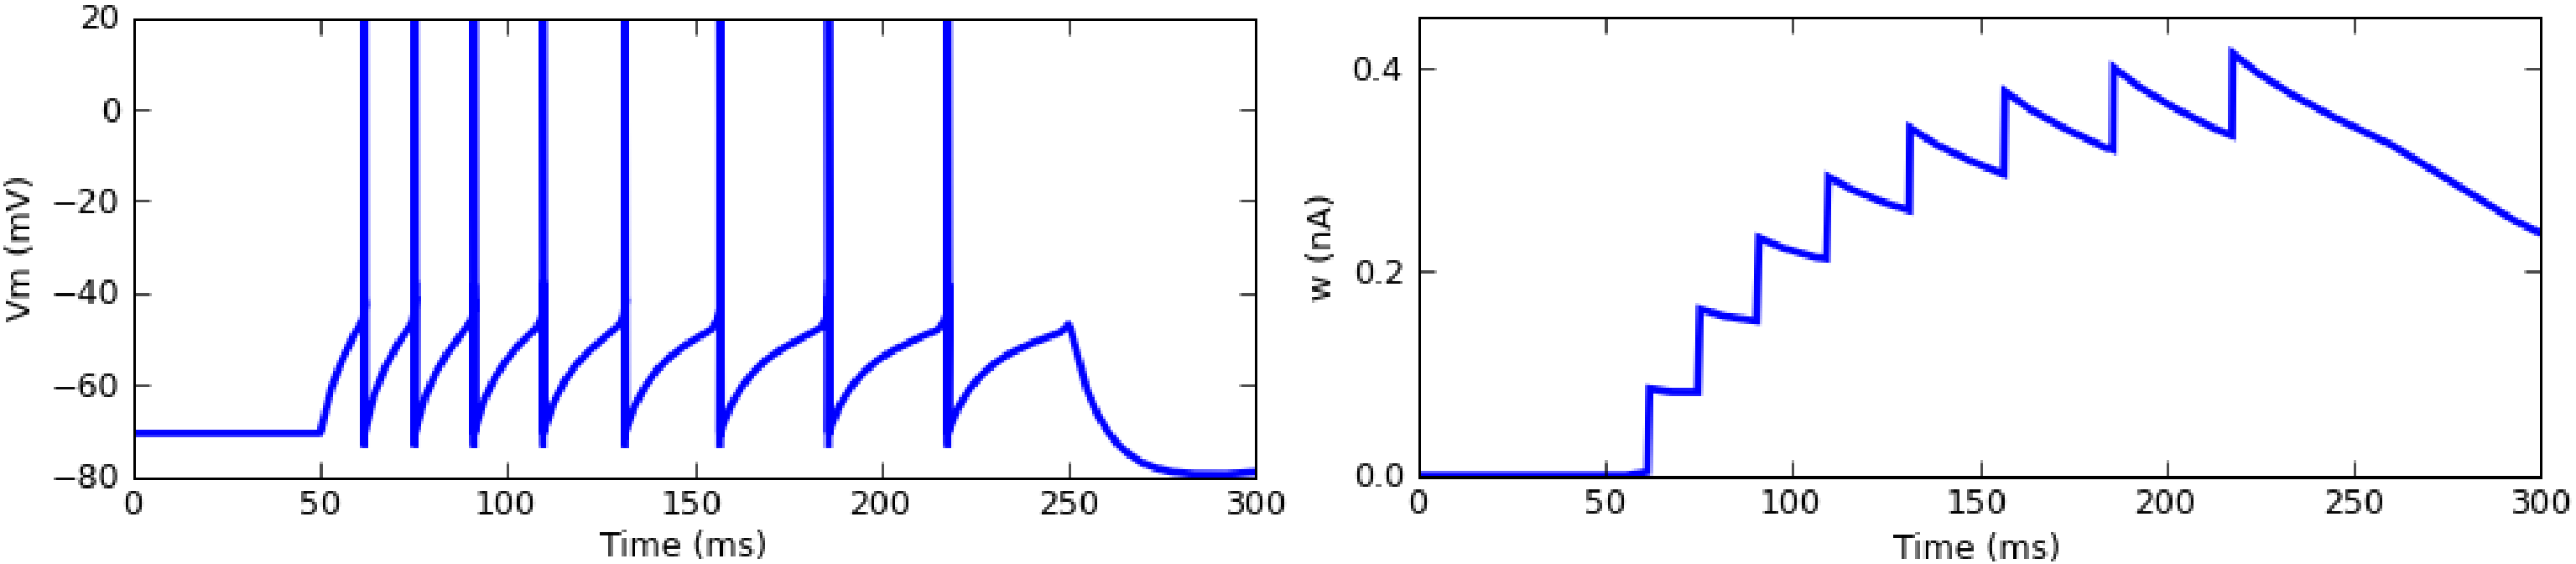
\includegraphics[scale=0.22]{10_9}
    \centering
\end{figure}
The AdEx neuron is also able to generate small bursts of activity by playing with the adaptation variable \(w\) and
the coupling parameter \(a\). Henceforth, with just a single model, it is possible to simulate several types of neurons,
by just properly tuning the parameters involved. Moreover, synapses can be added to build networks of AdEx neurons, even
studying the communication between clusters of AdEx neurons belonging to different families, thus exhibiting different
behaviours. Note that the AdEx neurons are highly compliant with the Hodgkin-Huxley model in terms of elicited activity.
\begin{figure}[H]
    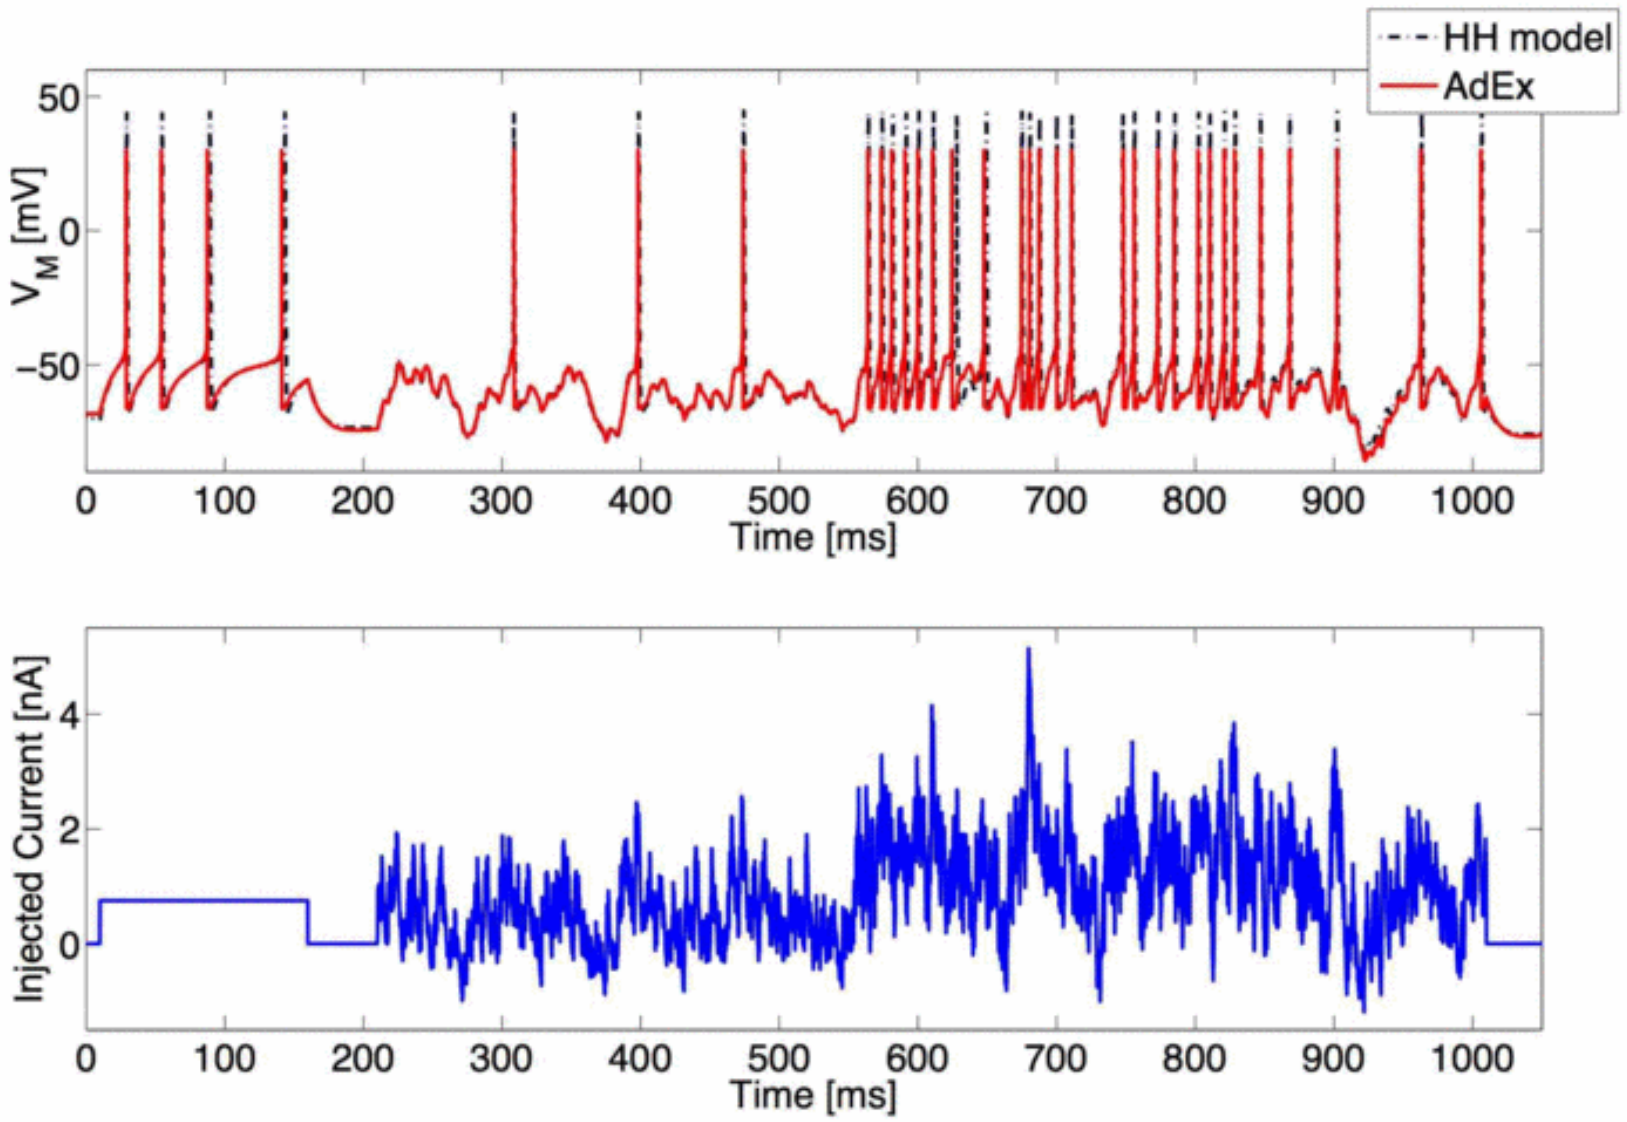
\includegraphics[scale=0.22]{10_10}
    \centering
\end{figure}
\subsubsection{Synapses in Integrate-and-Fire Neurons}
The effect of synapses can be taken into account in the models belonging to the Integrate-and-Fire family
by simply adding a term modelling the synaptic current:
\begin{equation*}
    C_{m}\frac{dV_{m}}{dt}=-g_{leak}(V_{m}-E_{leak})-\bar{g}_{syn}P_{syn}(V_{m}-E_{syn})+I_{app}
\end{equation*}
where \(P_{syn}\) is the probability release whenever the presynaptic neuron fires.

\subsection{The Izhikevich Model}
This model is based on bifurcation methodologies, which allow to reduce complex biophysically accurate models
such as the Hodgkin-Huxley one to 2D models:
\begin{align*}
    \frac{dv}{dt}&=0.04v^{2}+5v+140-u+I_{app}\\
    \frac{du}{dt}&=a(bv-u)
\end{align*}
where \(u\) is said to be the recovery variable and the after-spike resetting conditions are the following:
\begin{equation*}
    \text{if } v\ge{30\;mV}\rightarrow
    \begin{cases}
        v\leftarrow{c} \\
        u\leftarrow{u+d}
    \end{cases}
\end{equation*}
This model is especially appreciated due to its capability to simulate tens of different types of neurons,
each one with its peculiar characteristics and firing pattern, by just tuning the parameters in a
proper way. In addition, the values to be given to the model parameters in order to replicate the
activity of a certain kind of neuron are well defined, as reported in the following plots.
\begin{figure}[H]
    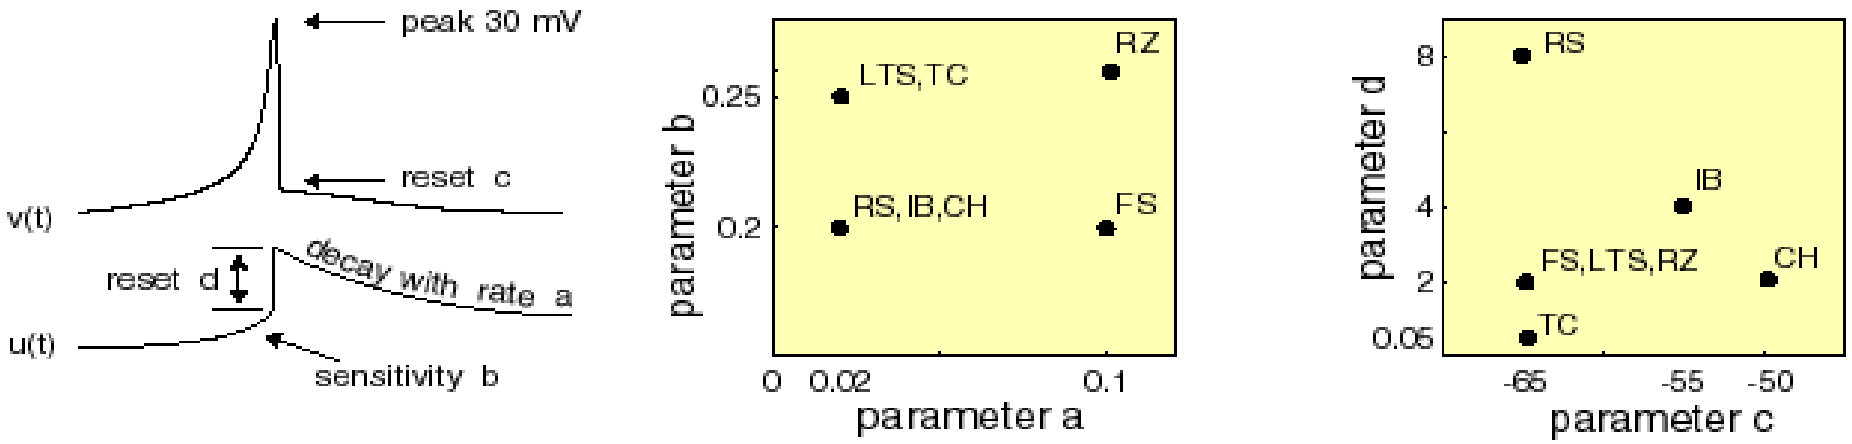
\includegraphics[scale=0.4]{10_11}
    \centering
\end{figure}
The parameters meaning is both illustrated in the figure above and described in this table:
\begin{center}
    \begin{tabular}{ |c|p{8cm}|c| }
        \hline
        \textbf{Parameter} & \textbf{Meaning} & \textbf{Typical Value} \\
        \hline\hline
        \(a\) & Describes the time scale of the recovery variable \(u\): small values imply a slow recovery. & \(0.02\) \\
        \hline
        \(b\) & Describes the sensitivity of the recovery variable \(u\) towards the sub-threshold fluctuations. & \(0.2\) \\
        \hline
        \(c\) & Describes the after-spike reset value of \(v\). & \(-65\;mV\) \\
        \hline
        \(d\) & Describes the after-spike reset value of \(u\). & \(2\) \\
        \hline
    \end{tabular}
\end{center}
Some of the activity patterns reproducible by exploiting the Izhikevich model are listed here.
\begin{figure}[H]
    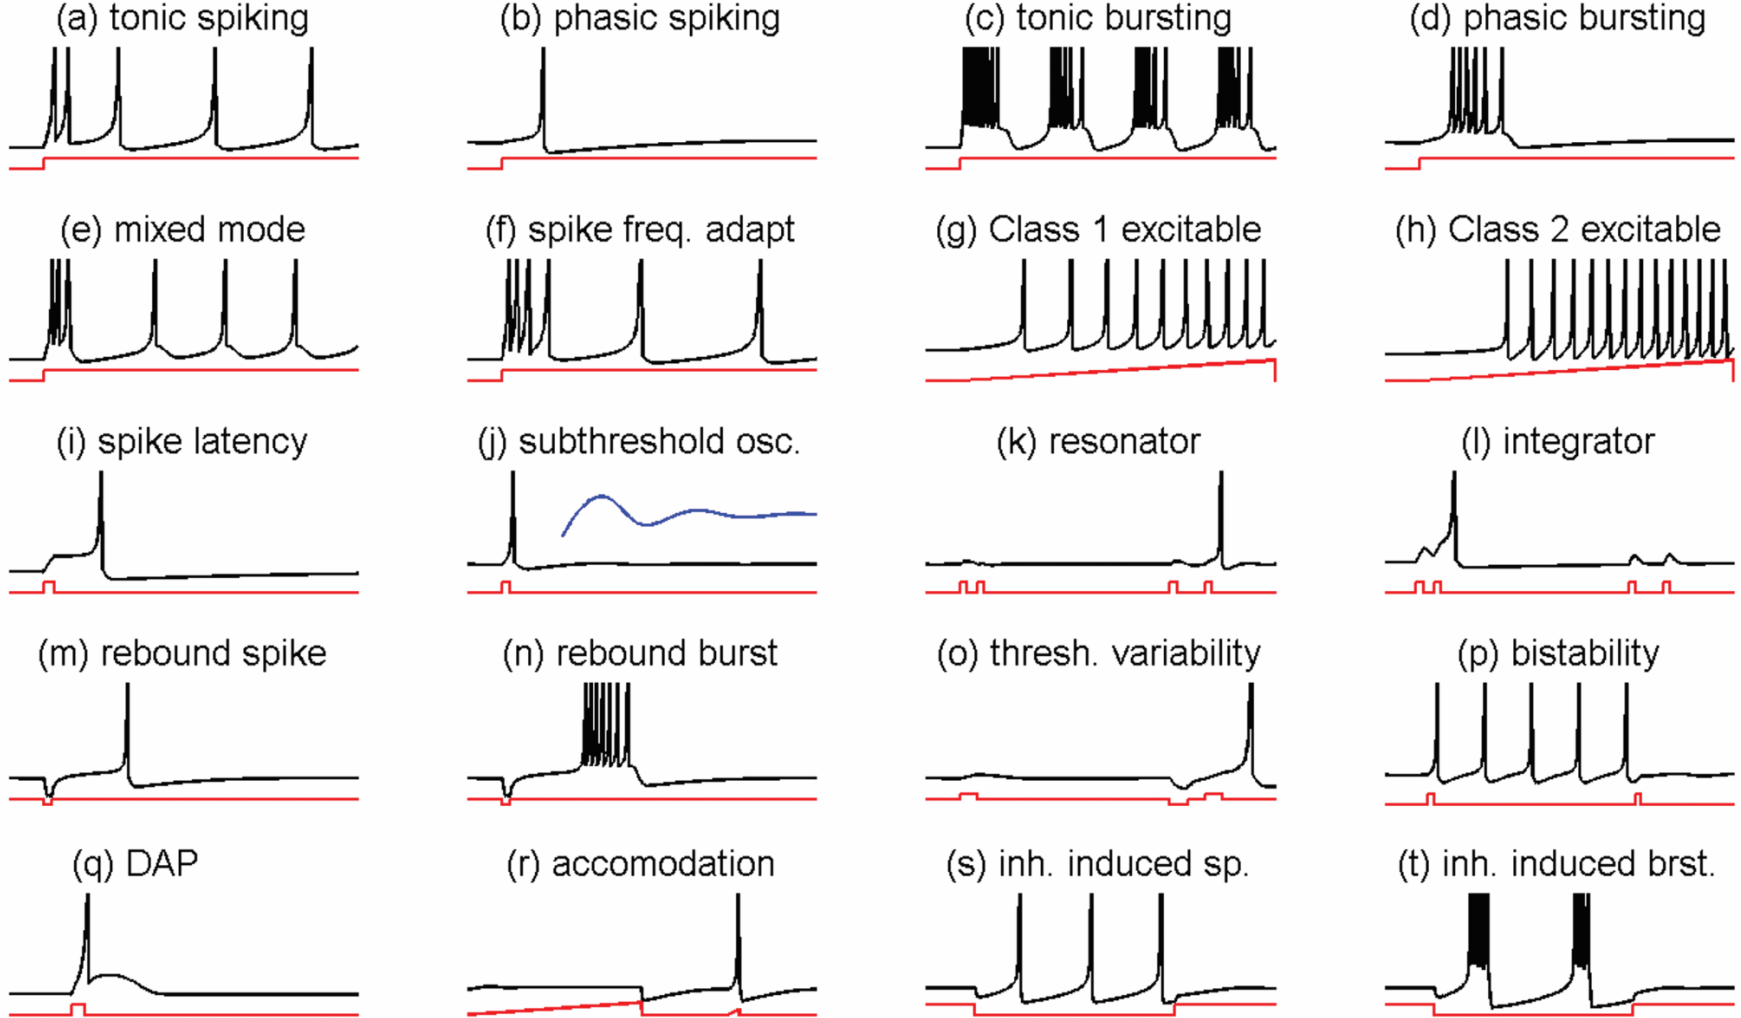
\includegraphics[scale=0.36]{10_12}
    \centering
\end{figure}
To sum up, several alternative models have been introduced in order to simulate the behaviour of
a neuron. The selection of the correct option is to be done by taking into account the goal of the
experiment: some models, as the HH one, are much better at reproducing also the shape of a single spike,
but in some cases such a degree of detail is not necessary, while a feasible computational cost is
a compulsory requirement, thus a model belonging to the IF family is to be preferred.

\subsection{Stochastic Point Process Models}
In some cases, researchers are not interested in simulating the whole activity of a neuron, but they
just need the sequence of spikes as a discrete time series of events, which is denominated spike
train.
\begin{figure}[H]
    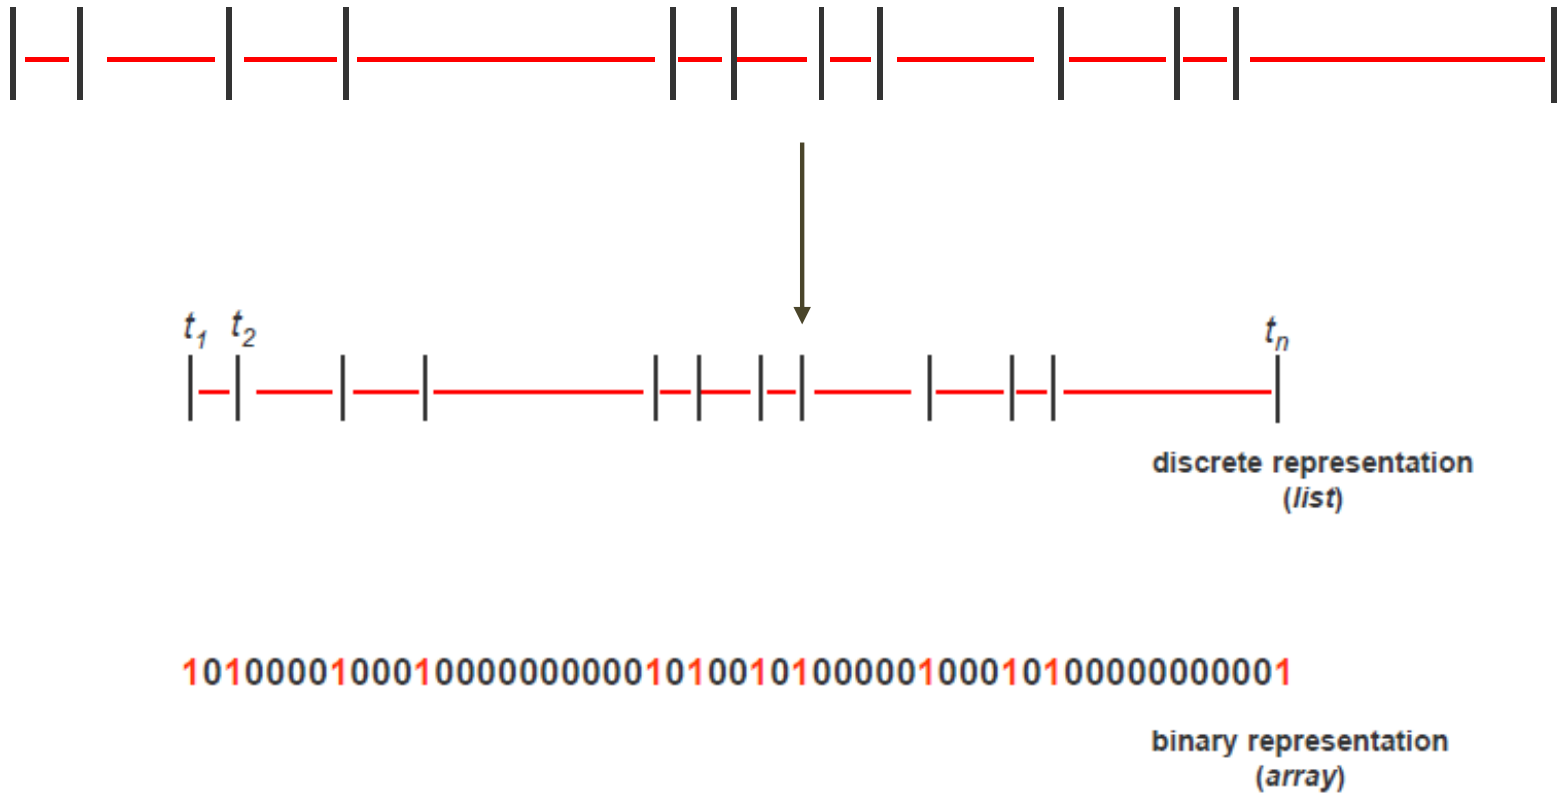
\includegraphics[scale=0.45]{10_13}
    \centering
\end{figure}
When dealing with stochastic point processes, there are two basic random variables involved:
\begin{itemize}
    \item \textbf{Inter-Event-Intervals}, such as ISI or IBI \(\Rightarrow\)
    \textit{continuous random variable}
    \item \textbf{Number of spikes} in a time interval \(T\) \(\Rightarrow\)
    \textit{discrete random variable}
\end{itemize}
Let's consider a point process defined in the \((-\infty;+\infty)\) domain. The history of
the process - i.e., a specification of the position of all points in the \((-\infty;t]\) interval -
is denoted by \(H_{t}\). Then, a general description of the process is given by the probability of
observing a single event at an arbitrary time \(t\):
\begin{equation*}
    P\bigl(N(t,t+\delta{t})=1|H_{t}\bigr)
\end{equation*}
In other words, this is the instantaneous probability to deliver a spike, depending on the time
\(t\) of the story of the process \(H_{t}\).
\subsubsection{Stationary Point Processes}
\paragraph{Poisson Process} A Poisson process of intensity \(\lambda\) is defined by the requirement
that \(\forall{t}\) and for \(\delta\to{0^{+}}\):
\begin{equation*}
    P\bigl(N(t,t+\delta{t})=1|H_{t}\bigr)=\lambda{\delta}+o(\delta)
\end{equation*}
Note that this is the only kind of process for which all the events are completely independent.
In addition, it is a simple process, which is often employed in the description of neural spiking.\\
The following plots represent two Poisson distributions with different value of \(\lambda\),
representing the ISI of the neuron.
\begin{figure}[H]
    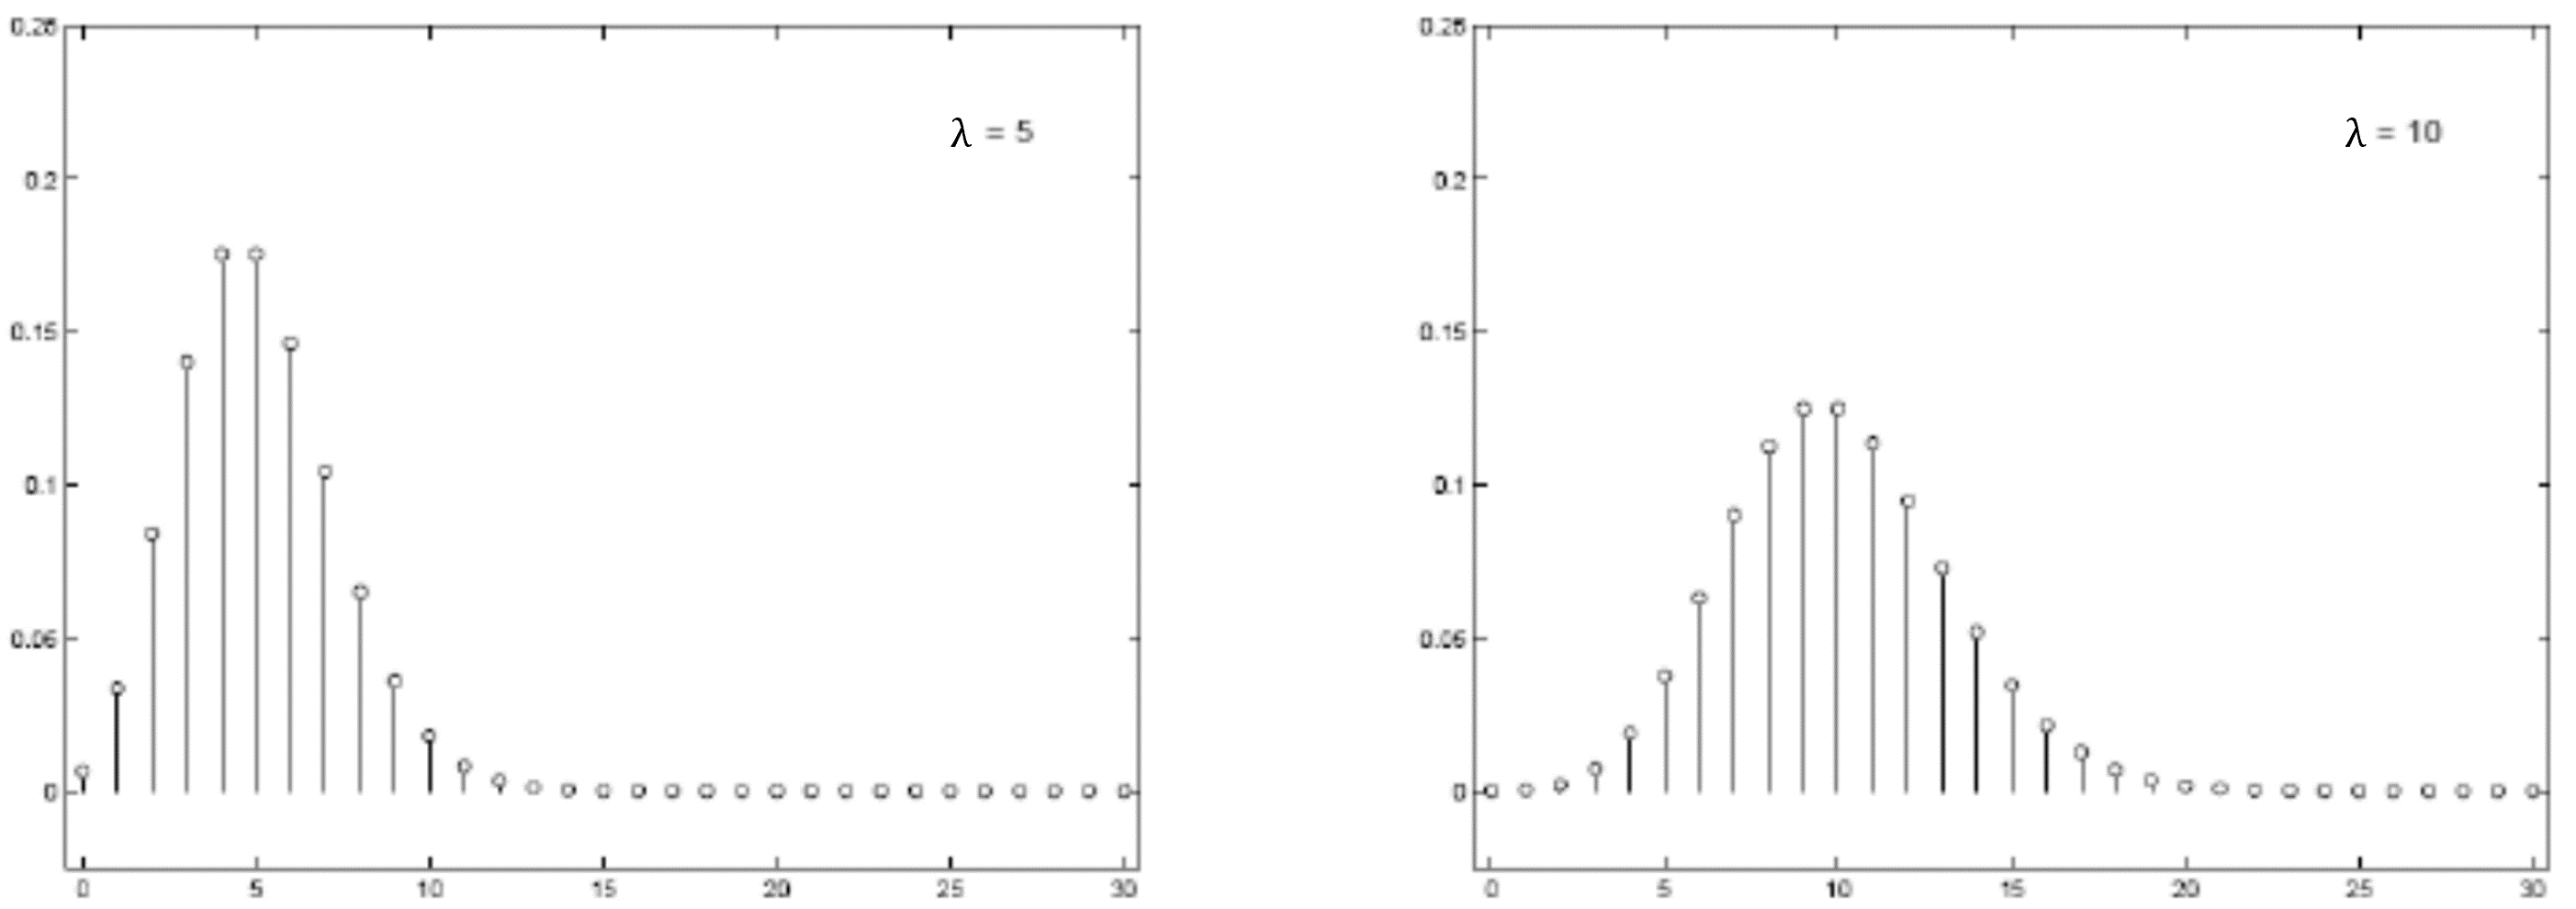
\includegraphics[scale=0.4]{10_14}
    \centering
\end{figure}
\paragraph{Renewal Process} In this kind of process the inter-event-intervals are independent
and identically distributed, therefore the process history is relevant only up to the previous
event. Note that the Poisson process is a specific type of renewal process.
\subsubsection{Non-Stationary Point Processes}
Non-stationary point processes are necessary as in experiments individual neurons can modulate
their firing rate with time, thus they do not fire in a stationary fashion. For instance, neural
plasticity modulates the generation of new spikes, as synapses are added and removed during the
ongoing activity.
\paragraph{Non-Homogeneous Poisson Process} Here the process intensity \(\lambda\) is no longer
constant, but it is a function of time, thus it becomes \(\lambda(t)\). Hence, the non-homogeneous
Poisson process model is defined by:
\begin{equation*}
    P\bigl(N(t,t+\delta{t})=1|H_{t}\bigr)=\lambda(t){\delta}
\end{equation*}
Note that the instantaneous probability is still independent on the process history.
\paragraph{Rate-Modulated Renewal Process} This model is equivalent to the renewal one, but
also here the process intensity \(\lambda(t)\) is varying over time.\\
\par
These models are especially useful when studying how the activity of some different populations
affect a target population, which is modelled by a more complex and computationally heavy solution,
such as the Izhikevich one. However, for the stimulationg populations, it is not important to fully
understand what is going in inside them, but the goal is to understand how the whole output,
such as a Poisson process, affects the target population.
